\subsection{Clinical discrimination from a recovered, identified score table}

The revised clinical analysis uses one row-level table of 4,677 identified
ClinVar variants across 20 genes. Complete official ESM-2 650M weights were
loaded in fp32, and wild-type-marginal LLRs were recomputed from the validated
reference sequences. All 24 full-sequence and windowed AUROCs reproduced the
saved corrected N6c summaries to their four-decimal precision. Repeated
full-sequence forwards were bitwise identical for all 20 genes in this run.
These are newly recovered scores, not scores inferred from AUROC targets.

Using the stated primary score (mutation-centred windows for sequences
longer than 1,024 residues), the mean per-gene AUROC is
\ClinicalMacroAUC{} (gene-resampling 95\% interval
$[\ClinicalMacroLow,\ClinicalMacroHigh]$; range 0.5571--1.0000).
Sixteen of 20 point estimates are at least 0.70 (Fig.~2).
Per-gene whiskers now use 2,000 class-stratified variant bootstrap draws,
replacing the unsupported historical intervals. For AICDA, perfect
separation of the 24 observed variants gives the expected empirical interval
$[1,1]$; this is not evidence of zero population uncertainty.
The saved gnomAD benign-source comparison remains a separately labelled
summary-level sensitivity (Fig.~2B and Fig.~S2). Its population-control
variants were not rescored in this revision. Gene exposure in sequence
pretraining and clinical ascertainment limit all of these comparisons to
the studied panel. Its saved mean gnomAD-minus-ClinVar AUROC difference is
$-0.019565$ (Fig.~S2); without paired uncertainty or newly recovered gnomAD
rows, this is a benign-source sensitivity, not a causal ascertainment
effect or transport test. The recovered table contains 1,108 pathogenic
and 3,569 benign variants; per-gene calibration bins, Brier scores and log-loss values
for these same rows are retained in the reproducibility exports accompanying
SI Table~S1. The discrimination and calibration results therefore refer to
one identified score version rather than to separate historical summaries.

\begin{figure}[!htbp]
\centering
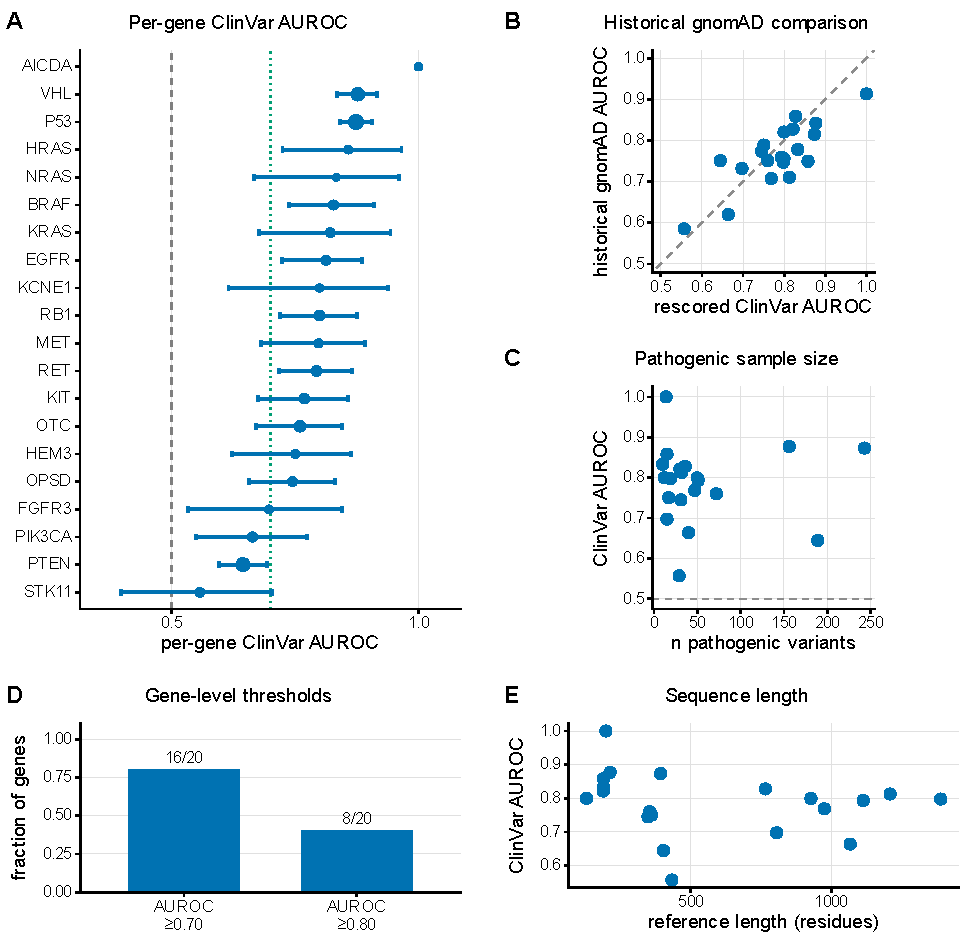
\includegraphics[width=\linewidth]{figures/F3_clinvar_forest.pdf}
\caption{{\bf Fig 2. Clinical discrimination from recovered fp32 scores.} (A) Per-gene AUROC for 4,677 variants across 20 genes, with 95\% percentile intervals from 2,000 class-stratified variant bootstrap draws; marker size indicates pathogenic sample size. AICDA's empirical interval is $[1,1]$ under perfect observed separation, not a claim of zero population uncertainty. Dashed and dotted lines indicate 0.5 and 0.70. (B) Newly recovered ClinVar AUROC versus the historical gnomAD-benign summary, not a newly rescored gnomAD cohort. (C) AUROC versus pathogenic sample size. (D) Point-estimate thresholds, 16/20 at AUROC $\geq0.70$ and 8/20 at $\geq0.80$. (E) Reference-sequence length versus AUROC. The new intervals are unadjusted per-gene summaries; no simultaneous significance or clinical-transport claim is made.}

\end{figure}

\subsection{Same-score calibration improves proper scores within the panel}

We next calibrated the same recovered LLRs with five-fold, class-stratified
cross-fitting, estimating all standardization and probability maps from
the fitting folds only. The sigmoid of the standardized negative LLR is
an arbitrary comparator, not a native model probability. Its pooled ECE
is \SigmoidECE{} and its Brier score is \SigmoidBrier{}.
Pooled Platt and tie-invariant isotonic maps reduce ECE to \PlattECE{}
and \IsoECE{}, with Brier scores \PlattBrier{} and \IsoBrier{}
(Fig.~3; Table~S1). Corresponding log losses are \PlattLogLoss{}
and \IsoLogLoss{}; the smaller isotonic ECE does not establish overall
superiority over Platt.

The fitting-fold pooled-prevalence baseline has ECE below $10^{-6}$ despite
a Brier score of \PooledPrevBrier{}. Class stratification makes that
near-zero pooled ECE unsurprising. A gene-prevalence baseline has Brier
score \GenePrevBrier{} and log loss \GenePrevLogLoss{}.
Thus low ECE alone does not imply useful variant discrimination. Relative
to this stronger gene-specific baseline, the paired Brier differences are
$-0.0105$ for Platt and $-0.0110$ for isotonic, with identity-grouped
refitting percentile ranges $[-0.0161,-0.0072]$ and
$[-0.0160,-0.0070]$, respectively. These differences support added
within-panel probability information beyond gene prevalence, conditional
on the observed gene and class composition.
The complete map-by-map OOF values and the identity-grouped refit summaries
are given in SI Tables~S1--S2. Table~S2 is part of the result chain because
the original OOF point, bootstrap mean and percentile range answer different
questions; the refit distribution is not a replacement confidence interval
for the fixed-fold point.

\begin{figure}[!htbp]
\centering
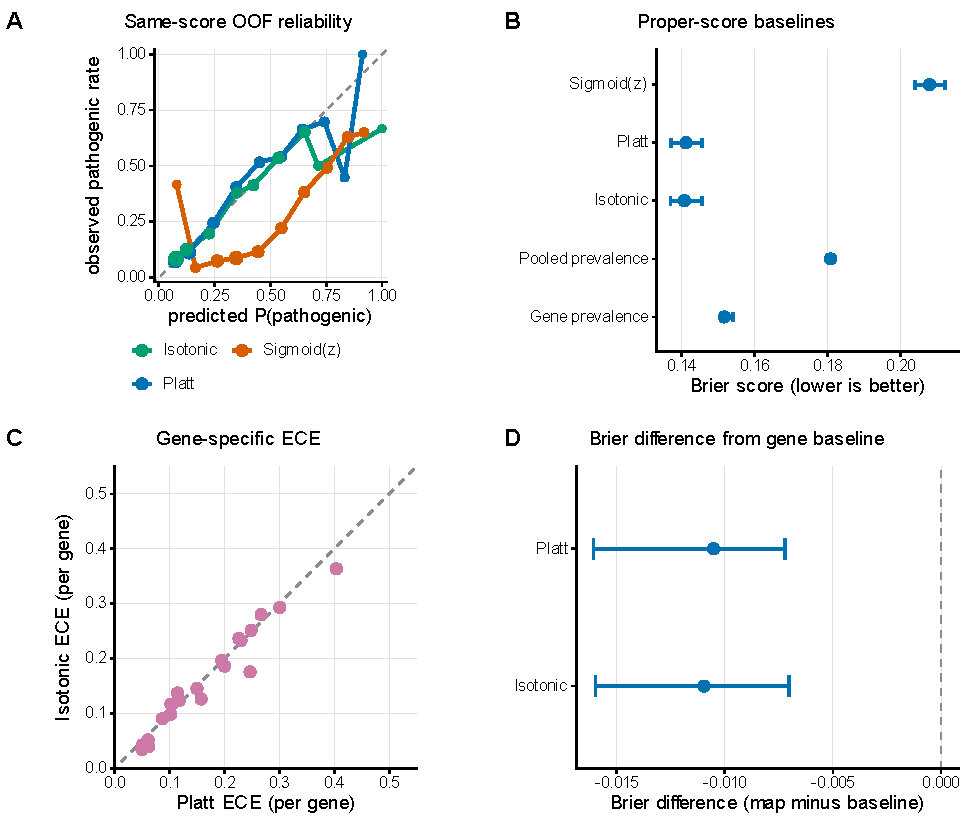
\includegraphics[width=\linewidth]{figures/F4_clinical_calibration.pdf}
\caption{{\bf Fig 3. Same-score, within-panel calibration with explicit baselines.} All panels use five-fold OOF predictions for the same 4,677 variants as Fig.~2 (seed 20260923). Standardization and calibrators use fitting folds only. (A) Ten equal-width reliability bins for sigmoid($z$), pooled Platt and tie-invariant isotonic maps; point size indicates bin count, and only occupied bins are connected. Sigmoid($z$) is not a native model probability. (B) Brier scores, including pooled- and gene-prevalence baselines fitted on the same training folds. (C) Per-gene ECE under the two calibrated maps, using these same OOF predictions; each point is one gene, not an independent calibration experiment. (D) Paired Brier differences from the gene-prevalence baseline. Whiskers in B and D are 2.5th--97.5th percentiles of 1,000 gene-by-class-stratified refitting draws, keeping each original variant in one fold and retaining bootstrap multiplicity. Points and refit distributions are reported separately and need not be centred. These are within-panel results, not gene/position holdout or clinical deployment validation.}

\end{figure}

\subsection{Uncertainty and version boundaries limit the clinical claim}

The 1,000 refitting draws resample within gene and class and preserve each
original variant's multiplicity without splitting its copies across
fitting and evaluation folds. This corrects bootstrap-copy leakage, but
is not a gene-, residue-position- or homology-disjoint evaluation. Pooled
calibration also does not guarantee calibration for each gene (Fig.~3C).
The percentile ranges describe the refitted bootstrap distribution, not
intervals centred on a fixed-fold point. For example, isotonic ECE is
0.0083 on the original OOF predictions, whereas its refit mean is 0.0159
and its 95\% percentile range is $[0.0090,0.0253]$. The difference is
reported rather than shifting the interval to include the point. The
first-half and second-half Monte Carlo ranges are retained in SI Table~S2,
and the per-gene reliability-bin coordinates are retained in the exports
used for Fig.~3. These supplemental records do not add a new clinical
population: they document the same 4,677 identified variants and the same
within-panel estimand.

The old calibration table had a mean per-gene AUROC of 0.6560, compared
with 0.7841 for the corrected scorer. Its six-gene reliability figure,
twenty-gene degradation counts, Cox/Holm analyses, selective-prediction
claims and decision-curve conclusions are not carried forward. They
remain historical audit records. The revised figures, intervals and
proper-score comparisons all derive from the recovered table.
Exploratory coverage and decision-curve coordinates are retained in the
reproducibility data, but do not establish a clinically chosen threshold,
external calibration or deployment benefit. Independent clinical
validation remains necessary.
